% Documentation for pkuthss.
%
% Copyright (c) 2008-2009 solvethis
% Copyright (c) 2010-2019 Casper Ti. Vector
%
% This work may be distributed and/or modified under the conditions of the
% LaTeX Project Public License, either version 1.3 of this license or (at
% your option) any later version.
% The latest version of this license is in
%   https://www.latex-project.org/lppl.txt
% and version 1.3 or later is part of all distributions of LaTeX version
% 2005/12/01 or later.
%
% This work has the LPPL maintenance status `maintained'.
% The current maintainer of this work is Casper Ti. Vector.
%
% This work consists of the following files:
%   pkuthss.tex
%   chap/pkuthss-copy.tex
%   chap/pkuthss-abs.tex
%   chap/pkuthss-intro.tex
%   chap/pkuthss-chap1.tex
%   chap/pkuthss-chap2.tex
%   chap/pkuthss-chap3.tex
%   chap/pkuthss-concl.tex
%   chap/pkuthss-encl1.tex
%   chap/pkuthss-ack.tex

\chapter{前言}	
\echapter{Introduction}
\section{夸克,胶子和强子}
\esection{Quarks, gluons and hadrons}

以下内容为范例:

夸克和胶子合称部分子,是自然界物质的基础组成部分。夸克之间存在强相互作用力,而色场中的胶子又能联系夸克组成强子,这个过程中的强相互作用能够统一地被量子色动力学(Quantum Chromodynamics, QCD)\parencite{Han:1965pf}所描述。量子色动力学属于非阿贝尔群规范理论\parencite{Gross1973UltravioletBO},其中有两个重要特征:

\begin{itemize}
	\item \textbf{色禁闭\parencite{GellMann:1964nj,Zweig:1964jf}}:喵喵喵
	\item \textbf{渐近自由}:喵喵喵
\end{itemize}

\section{夸克胶子等离子体(QGP)}
\esection{Quark-gluon Plasma}

\begin{figure}[htb]
	\centering
	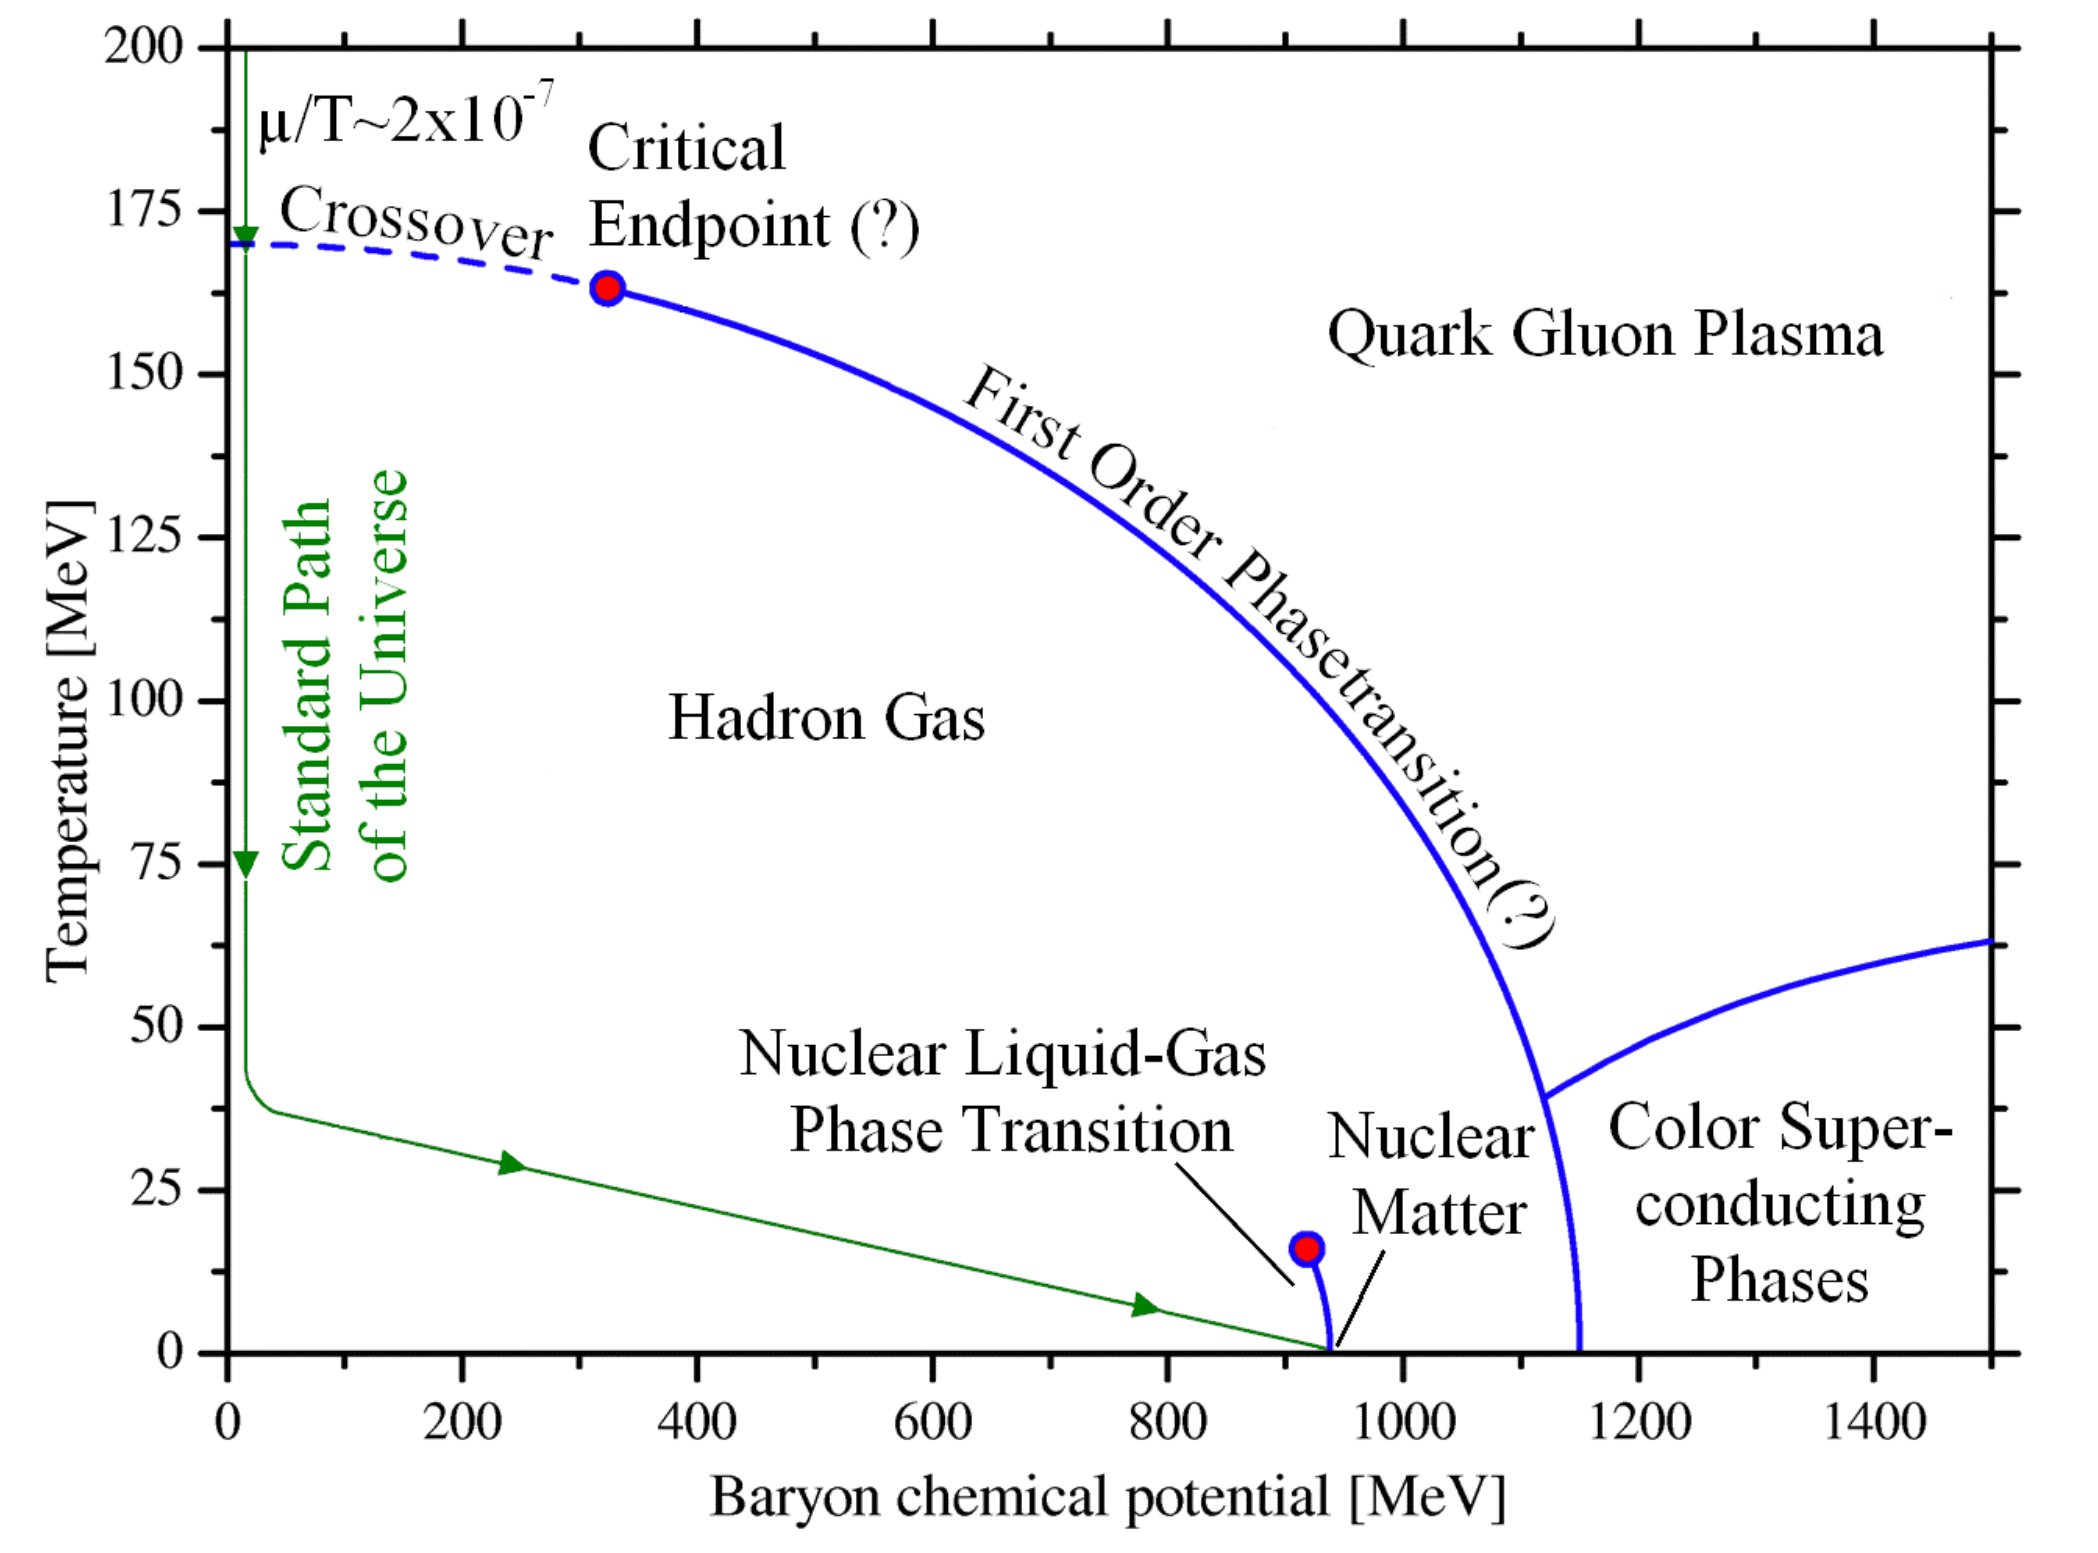
\includegraphics[width=0.7\linewidth]{../figures/1-thesis.png}
	\caption{量子色动力学核物质相变图。~\parencite{Boeckel:2011yj}}
	\label{fig:1-thesis}
\end{figure}

格点量子色动力学对核物质相变做了相关计算并预言了夸克胶子等离子体 ~\parencite{Shuryak:1978ij, Bohr:1977gj, Zajc:2007ey}的存在,QCD相图如图~\ref{fig:1-thesis}
所示,其中也包括许多理论计算推测。相图横轴是与净重子数成正比的净重子化学势,纵轴是温度。夸克胶子等离子体存在于高温(> 150 - 170 MeV)或是高净重子数密度条件下,所以产生QGP的方式既可以是提高核物质的温度,也可以是压缩其体积使净重子数密度提高,或者是两者同时进行。

\section{高能重离子碰撞}
\esection{High Energy Heavy-ion Collisions}

\section{集体流}
\esection{Collective Flow}

\subsection{各种流的现象体现}
\esubsection{Phenomena of Collective Flow}

\subsubsection{径向流(radial flow)}
\esubsubsection{Radial Flow}

\subsection{相对论流体力学模型}
\esubsection{Hydrodynamics Model}
QGP膨胀相关的动力学描述和集体流行为,可以通过量子色动力学的拉格朗日密度描述:

\begin{equation}
\mathit{L}=\overline{\Psi }_{i}(i\gamma_{\mu }\mathit{D}_{ij}^{\mu }-m\delta_{ij})\Psi_{j}-\frac{1}{4} \mathit{F}_{\mu \nu \alpha } \mathit{F}^{ \mu \nu \alpha}
\end{equation}

其中$\Psi_{i}$指夸克场($i$对应不同的色荷状态),$\mathit{D}^{\mu}$是协变导数,$m$是夸克质量,$ \mathit{F}^{ \mu \nu \alpha}$是胶子对应的场强张量,其中$\alpha$对应胶子的色荷状态。

\section{小系统中的集体流行为}
\esection{Collectivity in Small System}

\section{文献综述和论文结构}
\esection{Thesis Structure}


% vim:ts=4:sw=4
